%% 歩容パターンの再評価手法の提案.tex
%% LaTeX-2e 専用

%% 全体の流れとしては,まず,先行研究の問題点を指摘し,次に,歩容パターンの再評価手法を提案する.

\chapter{歩容パターンの再評価手法の提案}\label{chapter:歩容パターンの再評価手法の提案}
第\ref{chapter:歩容パターンの再評価手法の提案}章では,先行研究の手法およびその問題点を指摘し,
常に脚軌道生成が可能な自由歩容パターン生成手法として,歩容パターンの再評価手法を述べる.

% 先行研究の章
\section{本研究室における自由歩容パターン生成の先行研究}
\subsection{グラフ理論について}
グラフとは,頂点(ノード)とそれらを結ぶ辺(エッジ)からなる図形である.
このグラフを用いて,さまざまな問題を取り扱う学問をグラフ理論という.

以降の説明を簡単にするため,この論文で用いるグラフ理論の用語について簡潔に述べる.
エッジに向きがあるものを有向グラフ,逆に向きを持たないものを無向グラフという.
また,閉路を持たず,かつ,すべての頂点間に経路が存在するグラフを木という.
このような木構造をもつグラフのうち,図\ref*{fig:tree_graph}のように,
根となるノードを持ち,そのノードからすべてのノードに到達可能なものを根付き木という.

根付き木において,あるノードから遷移可能なノードをそのノードの子ノードと呼ぶ.
逆に,あるノードに遷移可能なノードをそのノードの親ノードと呼ぶ.
親ノードを持たないノードを根ノードと呼び,子ノードを持たないノードを葉ノードと呼ぶ.
また,あるノードから根ノードまでのエッジの数をそのノードの深さと呼び,
根ノード自身の深さは0となる.

図\ref*{fig:tree_graph}においては,ノードAが根ノードであり,ノードB,Cがその子ノードである.
また,ノードB,ノードD,E,ノードCはノードFを子ノードとして持ち,ノードD,E,Fは葉ノードである.
ノードAの深さは0であり,ノードB,Cの深さは1,ノードD,E,Fの深さは2となる.

グラフのあるノードから別のノードに到達するための経路をパスと呼び,
これを求めることをグラフ探索と呼ぶ.
グラフ探索には,深さ優先探索,幅優先探索などのさまざまなアルゴリズムが存在する.
深さ優先探索では,始点となるノードから,深さが深くなる方向を優先して探索を行う.
これに対して,幅優先探索では,始点となるノードから,深さが浅いノードを優先して探索を行う手法である.

\begin{figure}[tbp]
  \begin{center}
    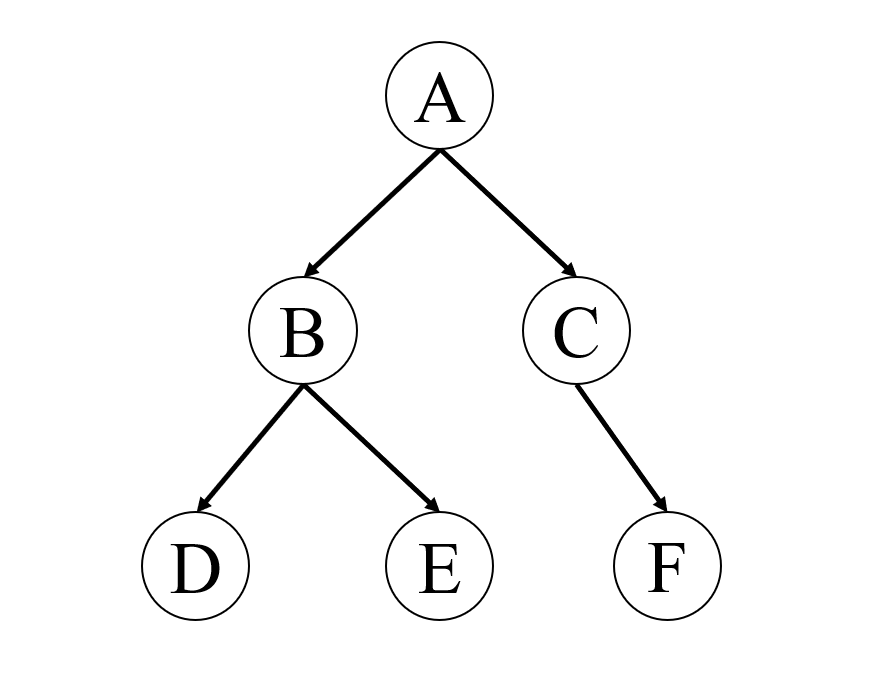
\includegraphics[width=50mm, clip]{figure/tree_graph.png}
   \caption{Tree Graph}
    \label{fig:tree_graph}
  \end{center}
\end{figure}

\subsection{歩容パターングラフについて}
本研究においては,6脚ロボットの歩容パターンをグラフを用いて表現する.
ロボットの状態をノードとし,ロボットの状態間の遷移,つまりロボットの動作をエッジとして表現する.
また,グラフは有向の根付き木とする.このようにして作られたグラフを歩容パターングラフと定義する.

グラフ探索がよく用いられる題材は路線図や回路図などであり,ノードの数が有限であるものである.
しかし,歩容パターングラフはロボットの状態や動作を対象とするため,
無限の組み合わせが存在する.そのため,状態や動作を離散化する必要がある.

\subsection{脚軌道生成の失敗}


% 予備実験の章
\section{歩行シミュレーションによる脚軌道生成失敗時の脚先位置の特定}

\subsection{シミュレーション実験の目的}
脚軌道生成の失敗を防ぐためには,脚軌道生成の失敗時の脚先の座標を特定する必要がある.
そのため,予備実験として先行研究と同じ条件で歩行シミュレーション実験を行い,失敗の原因を考察した.

\subsection{シミュレーションの条件}

\subsection{シミュレーションの結果}
以下の図に脚軌道生成失敗時の脚先の座標を示す.

\subsection{脚軌道生成の失敗の原因の考察}

\section{常に脚軌道生成が可能な自由歩容パターン生成手法の検討}
常に脚軌道生成を可能にするためには,近似された脚可動範囲を適切に設定する必要がある.


\section{歩容パターンの再評価手法}

